\section{Scénario}

Pour simplifier, dans la suite du rapport nous considérons être sur un monoprocesseur
avec trois tâches: A, B et C. L'objectif présenté par les scénarios est de favoriser
la ou les tâches qui détiennent un verrou pour débloquer rapidement le fil d'exécution
des autres tâches potentiellement en attente, tout en ne dénaturant pas les principes
clés du CFS.


\subsection{Charge}

Une première solution est d'introduire un système de charge à chaque verrou, afin
d'influencer sa priorité.

\subsubsection{Augmentation de la priorité}

Considérons que les tâches A et C ont une priorité de 120 et B une priorité de 100.
La tâche A détient un verrou. Le scheduler doit favoriser A par rapport à C sans pour
autant être un inconvénient pour B.
Une augmentation de la priorité d'une valeur de 10 est un bon compromis. La tâche A
devient alors plus prioritaire que C sans dépasser B.
\\

Cependant, si C détient lui aussi un verrou, et que A et C bloquent respectivement 
10 et 100 tâches, alors augmenter la priorité de 10 au deux tâches semble non équitable
étant donné que C bloque plus de tâches que A. Ainsi, une augmentation dans un
intervalle de 0 à 10 est plus cohérent. La tâche A aura une priorité augmentée
de 2 contre 10 pour C. Cette augmentation de priorité sera déterminé
avec un système de \textbf{charge}.
\\

Une autre solution aurait pu être de modifier directement la valeur \verb|vruntime|
pour forcer la tâche à être à gauche de l'arbre \verb|rbtree| et ainsi assurer sa
réélection. Cependant, cela implique que la tâche passera devant tous les autres tâches,
y compris celles plus prioritaires. Cette solution écrase toute la logique du système
de priorité mis en place par le scheduler et donc n'a pas été retenue.


\subsubsection{Calcul de charge}

Chaque tâche propriétaire d'un verrou se verra attribuer une charge, celle-ci évoluera en fonction
des tâches bloquées sur le verrou. Plus une tâche a une charge élevée, plus sa priorité augmente.
\\

L'implémentation du calcul de charge est assez simple. 
La charge correspondra au nombre total de tâches couramment bloquées sur le verrou. 
Ainsi, la priorité ajoutée sera dans l'intervalle de 0 à 10 mais fonctionnera par
paliers en fonction de la charge: sur des échelons restant encore à définir, on peut
envisager que toutes les 5 tâches bloquées la priorité se voit augmenter de 1,
plafonnant ainsi l'augmentation à 50 tâches bloquées.
\\

Une autre implémentation aurait été de calculer cette charge avec un système 
de pourcentage. Un compteur qui, au fur et à mesure de la vie d'exécution de la
tâche A, compterait le nombre total de tâche qui peut potentiellement se bloquer
sur son verrou. Un deuxième compteur, indiquant le nombre de tâches actuellement
bloquées, permettrait de calculer un pourcentage de charge. Une simple division
par 10 de la charge aurait permis de calculer l'augmentation de la priorité. Mais
le pourcentage de charge n'est pas très parlant. Reprenons l'exemple précédent
où A et C bloquent respectivement 10 et 100 tâches avec maintenant une charge 
de 100\%.
Bien que C devrait être plus favorisé, il n'en reste que A et C auront toutes 
les deux une priorité augmentée de 10.


\subsubsection{Héritage de charge}

Pour rendre le système de charge plus efficace nous introduisons un héritage
de charge entre les tâches. Considérons que A détient un verrou et se bloque
en essayant de prendre un deuxième verrou détenu par B. Alors B verra sa
charge augmenter par la valeur celle de A. Ainsi, la tâche B sera plus favorisée même
si A et B ont la même priorité et la même charge au départ.
\\

L'héritage de charge est très utile mais demande aussi d'être très précis.
En effet, si la charge d'une tâche est incorrecte par rapport à la réalité
(i.e. la valeur ne correspond pas au nombre de tâches bloquées)
alors l'héritage ne peut qu'aggraver l'erreur. Il est très important
de s'assurer que la charge est valide en la décrémentant lorsqu'une tâche 
n'attend plus sur le verrou, notamment lorsque la tâche meurt avant de l'avoir pris.


\subsection{Héritage de priorité}

Un deuxième mécanisme est l'héritage de priorité. 
Considérons pour simplifier deux fils d'exécution
(tâche A et C) qui partagent le même espace d'adressage et qui veulent accéder 
à une même section critique, et un processus (tâche B) qui contient 
un seul fil d'exécution indépendant des deux 
premiers, dont les priorités sont définies comme ceci: Pri(C) $>$ Pri(B) $>$ 
Pri(A), même en considérant l'augmentation de priorité définie précédemment.
\\

NB: cette configuration peut être aussi atteignable avec 3 processus dont deux 
utilisent un segment de mémoire partagé ou bien 3 threads d'un même processus.
\\

Si la tâche A, qui se trouve être la moins prioritaire, prend un futex et que 
la tâche C, qui est la plus prioritaire, veut aussi l'acquérir, elle
devra se bloquer en attendant que la tache A libère le verrou. Étant donné que 
la tâche B possède une priorité plus élevée que le propriétaire du futex, elle 
sera choisie plus fréquemment par le scheduler. Ce comportement va ralentir 
l'exécution de la tâche C, la plus prioritaire, qui est bloquée en attente de la 
libération du futex par la tâche A.

\begin{figure}[h!]
	\centering
	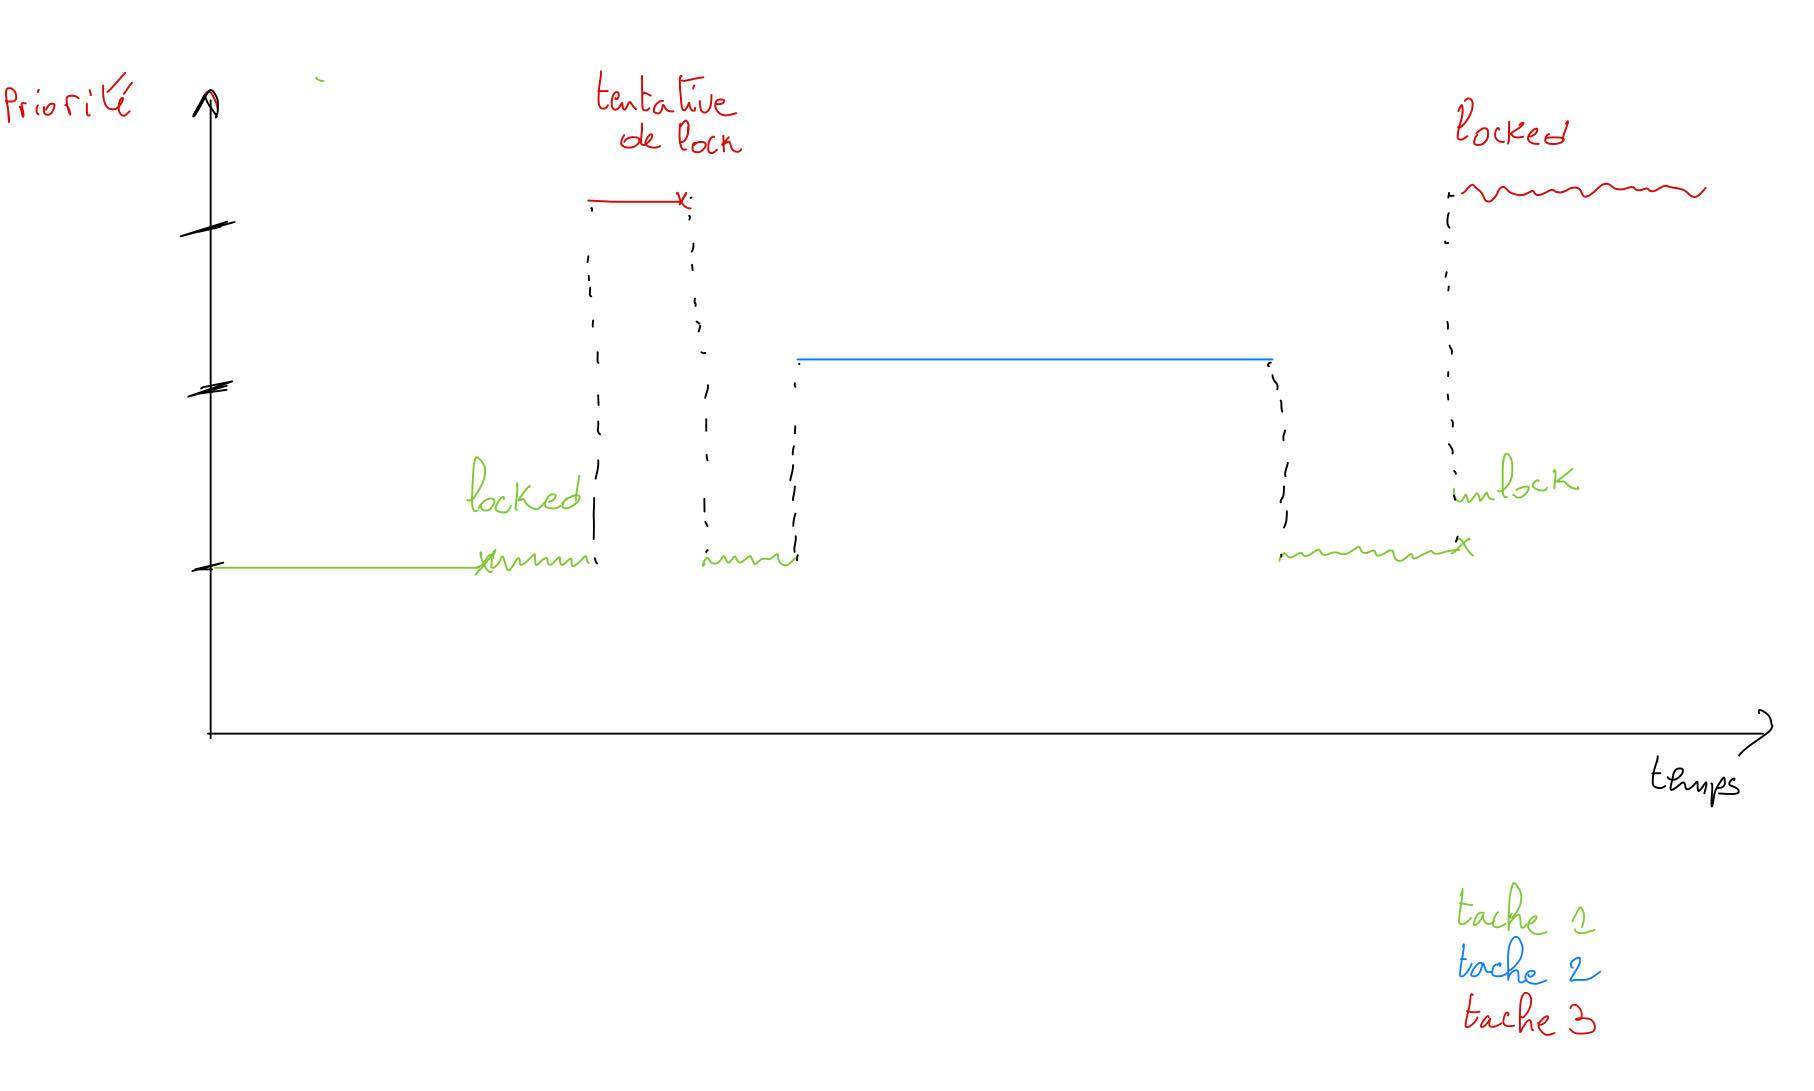
\includegraphics[scale=0.15]{include/without_inherit.jpg}
	\caption{Avancement des processus sans l'heritage de priorité}
	\label{fig:without_inherit}
\end{figure}

\newpage


L'idée ici est de modifier la priorité de la tâche A pour qu'elle soit plus 
prioritaire que la tâche B. On peut atteindre cela en héritant de la 
priorité de la tâche C, qui est plus prioritaire que la tâche B. 
\\

Ainsi, le propriétaire du verrou se verra attribuer, au cours de son exécution, 
la priorité de la tâche la plus prioritaire parmi toutes les tâches bloquées 
sur le verrou. De plus, l'augmentation de la priorité par rapport à la charge 
introduite précédemment sera appliquée à cette nouvelle priorité.
\\

\begin{figure}[h!]
	\centering
	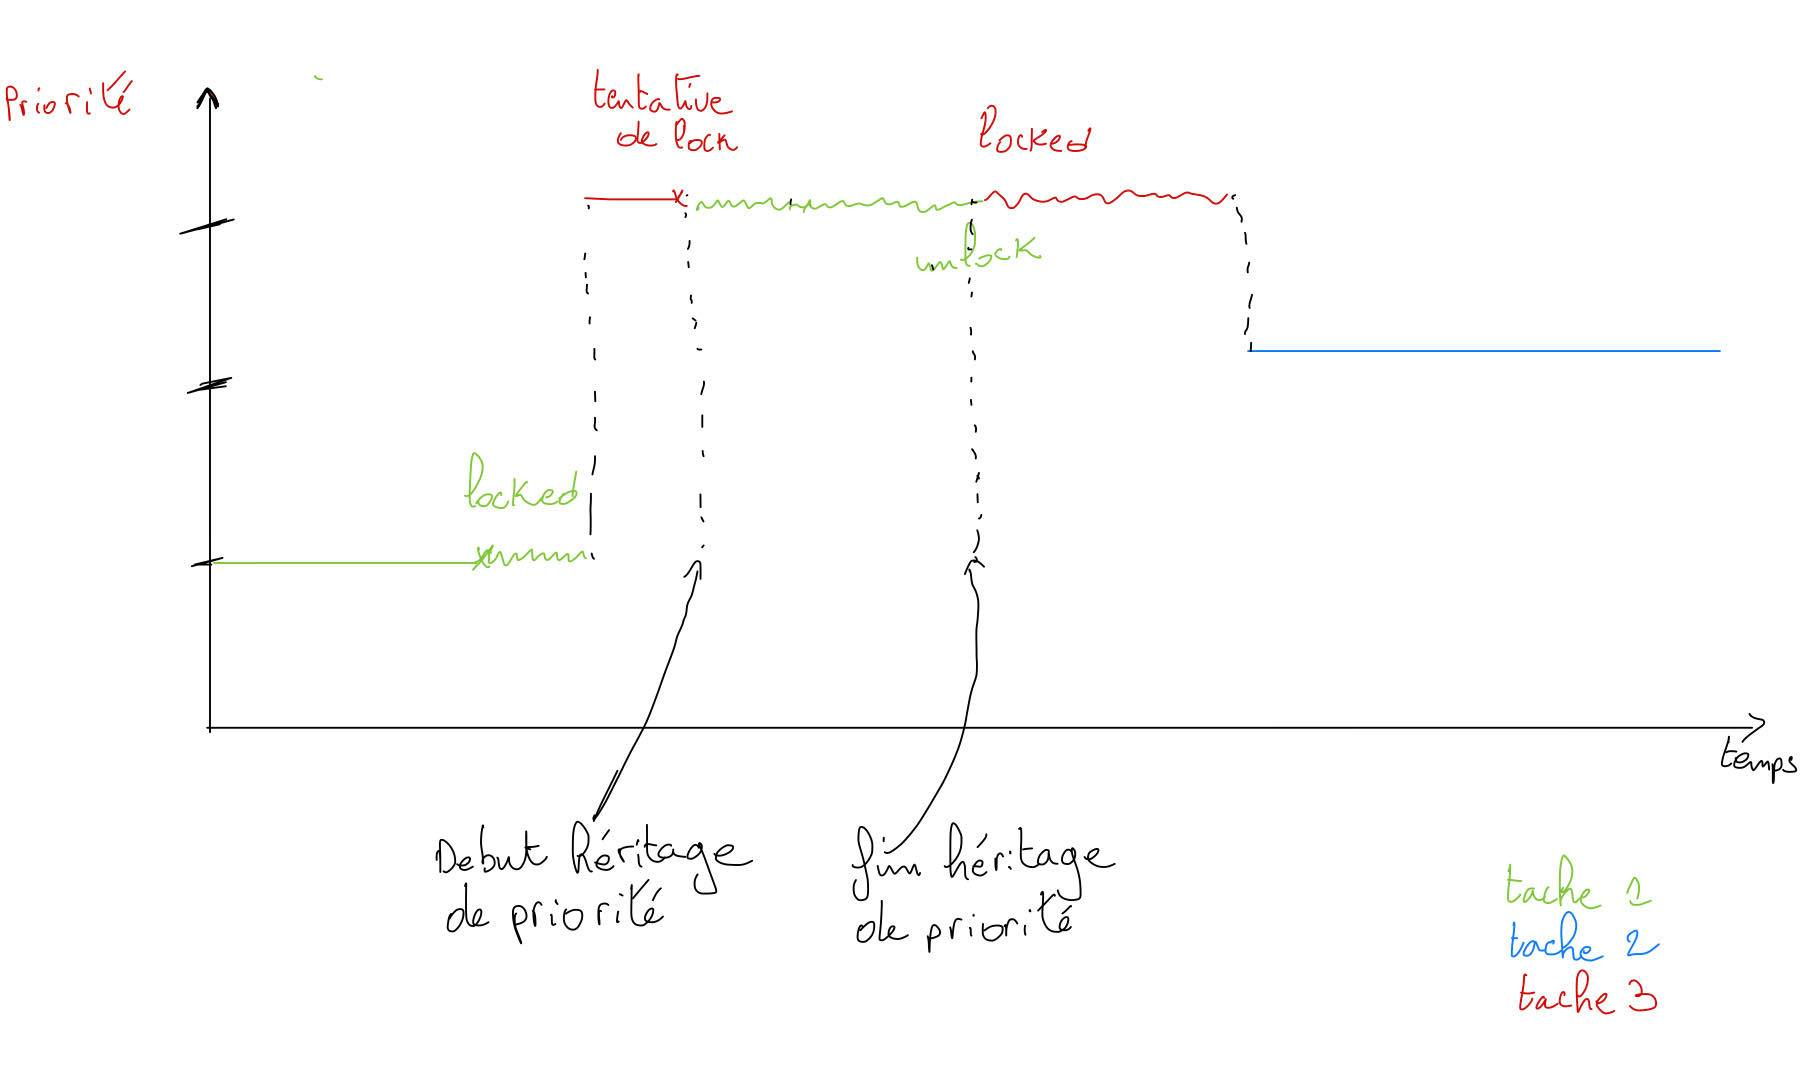
\includegraphics[scale=0.15]{include/with_inherit.jpg}
	\caption{Avancement des processus avec l'heritage de priorité}
	\label{fig:with_inherit}
\end{figure}


Le CFS est connu pour être un scheduler très équitable, en combinant ces deux techniques cela permet d'assurer une implémentation qui reste juste pour chaque tâche.